%%%%%%%%%%%%%%%%%%%%%%%%%%%%%%%%%%%%%%%%%
% Sleek, Extensible Journal Article
% LaTeX Template
% Version 0.1
% Date 01/05/2014
%
% Original author:
% Calem Bendell
%
% License:
% CC BY-NC-SA 3.0 (http://creativecommons.org/licenses/by-nc-sa/3.0/)
%
%%%%%%%%%%%%%%%%%%%%%%%%%%%%%%%%%%%%%%%%%

\documentclass[10pt, twocolumn]{scrartcl}
\usepackage[T1]{fontenc}

\usepackage{lipsum}

\usepackage{kpfonts}
\usepackage{helvet}
\linespread{1.05}
\usepackage{microtype}

\usepackage[top=5em, left=5em, right=5em, bottom=7em, columnsep=2em]{geometry}
\usepackage[hang, small,labelfont=bf,up,textfont=it,up]{caption}
\usepackage[hidelinks, colorlinks=true]{hyperref}
\usepackage{booktabs, float, paralist, titlesec, abstract, titling, enumitem, graphicx}
\usepackage[usenames,dvipsnames,svgnames,table]{xcolor}
\usepackage[flushmargin,hang,multiple]{footmisc}
\interfootnotelinepenalty=10000

\renewcommand{\abstractnamefont}{\normalfont\large\sffamily}
\renewcommand{\abstracttextfont}{\normalfont\itshape}

\titleformat*{\section}{\Large\sffamily}
\titleformat*{\subsection}{\large\sffamily}
\titleformat*{\subsubsection}{\itshape\sffamily}
\titleformat*{\paragraph}{\large\bfseries\sffamily}
\titleformat*{\subparagraph}{\large\bfseries\sffamily}

\setlist[description]{format=\normalfont\itshape}

\renewcommand{\maketitle}{\noindent\rule{\linewidth}{1pt}\huge \vspace{1em} \newline
\sffamily \scshape \thetitle \\
\normalfont \sffamily  \theauthor \\
\thedate
\newline\noindent\rule{\linewidth}{1pt}
\vspace{1em}
\normalfont
\normalsize}


\title{Savings Report for Laboratory: \vspace{.1em} \\  Otto Mass Building 119 Room 230}
\author{
\large
{ Equipmind of Glencross Brunet Inc \\
\normalsize \href{mailto:calem@equipmind.com}{calem@equipmind.com}
}
}
\date{}

\begin{document}
\twocolumn[\maketitle

\begin{abstract}
	This is a report made for you for this particular lab should you want a more in depth analysis of the results we gathered for your laboratory.
	In particular, the method by which we generated your results is presented.
\end{abstract}]

\section{Glossay of Terms}

	\begin{description}
		\item[Fumehood ] HyveDev is the name for the automation team outside of Solar Decathlon.
	\end{description}

\section{Introduction}

\section{Method}

\section{Data}

	\begin{figure*}
		\centering
		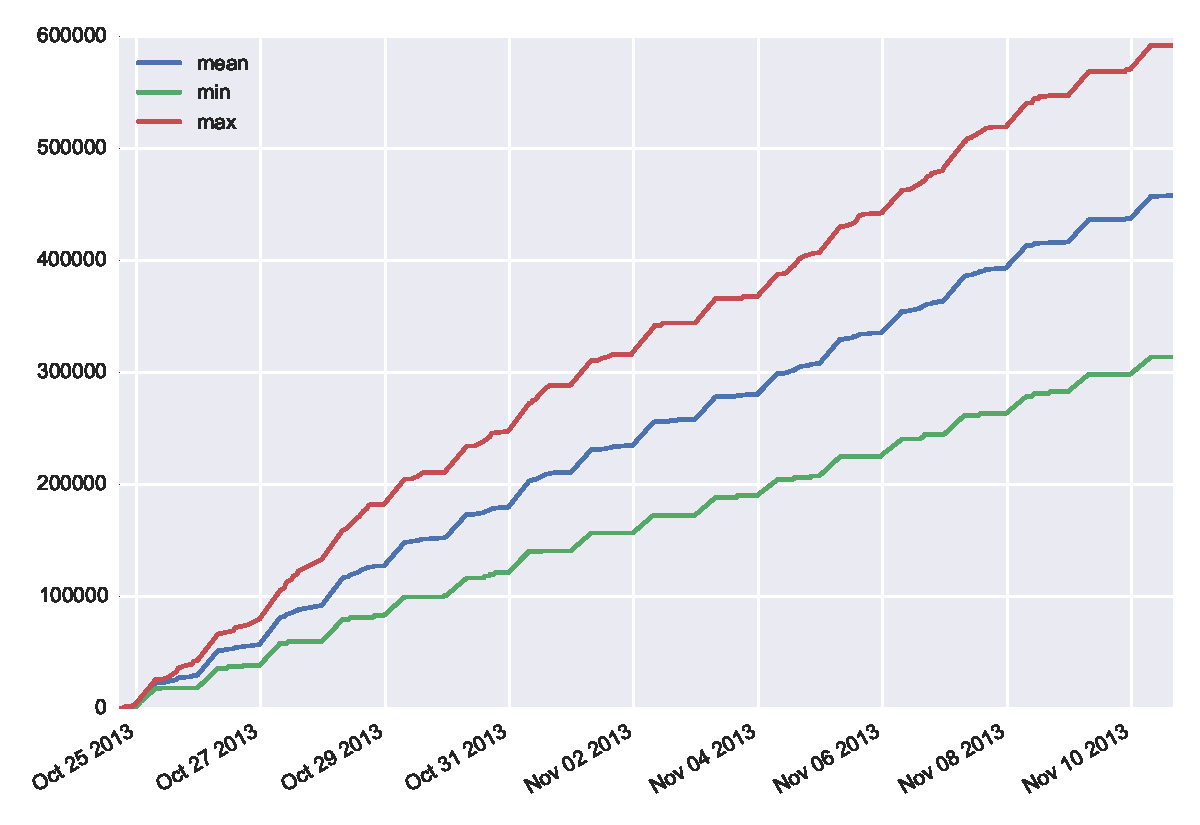
\includegraphics[width=\textwidth]{savings_summary.pdf}
		\caption{A summary of the cumulative savings of a laboratory across the different parameters tested.}
	\end{figure*}

	\begin{figure*}
		\centering
		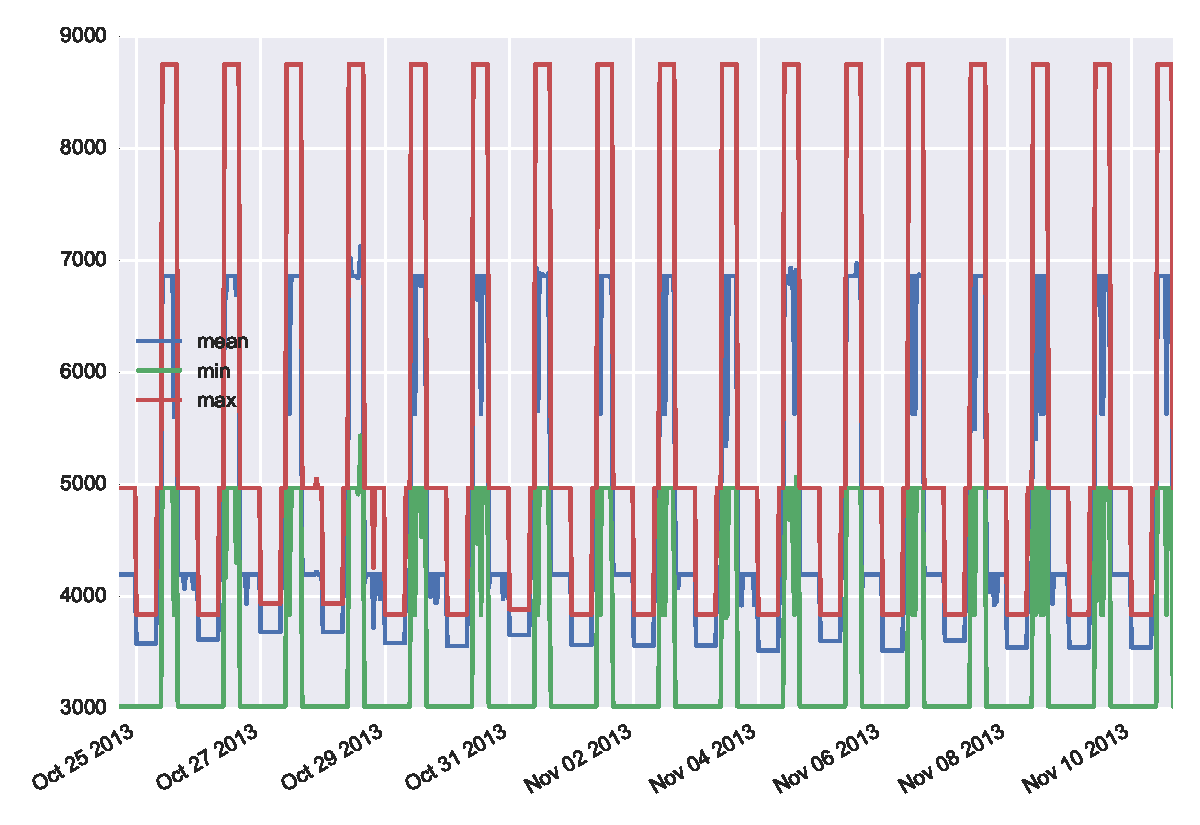
\includegraphics[width=\textwidth]{adjusted_sums_summary.pdf}
		\caption{A summary of the summation of all fumehood and laboratory evacuation over time across the different parameters evaluated.  Significant dips in evacuation are typically night time.}
	\end{figure*}

	\begin{figure*}
		\centering
		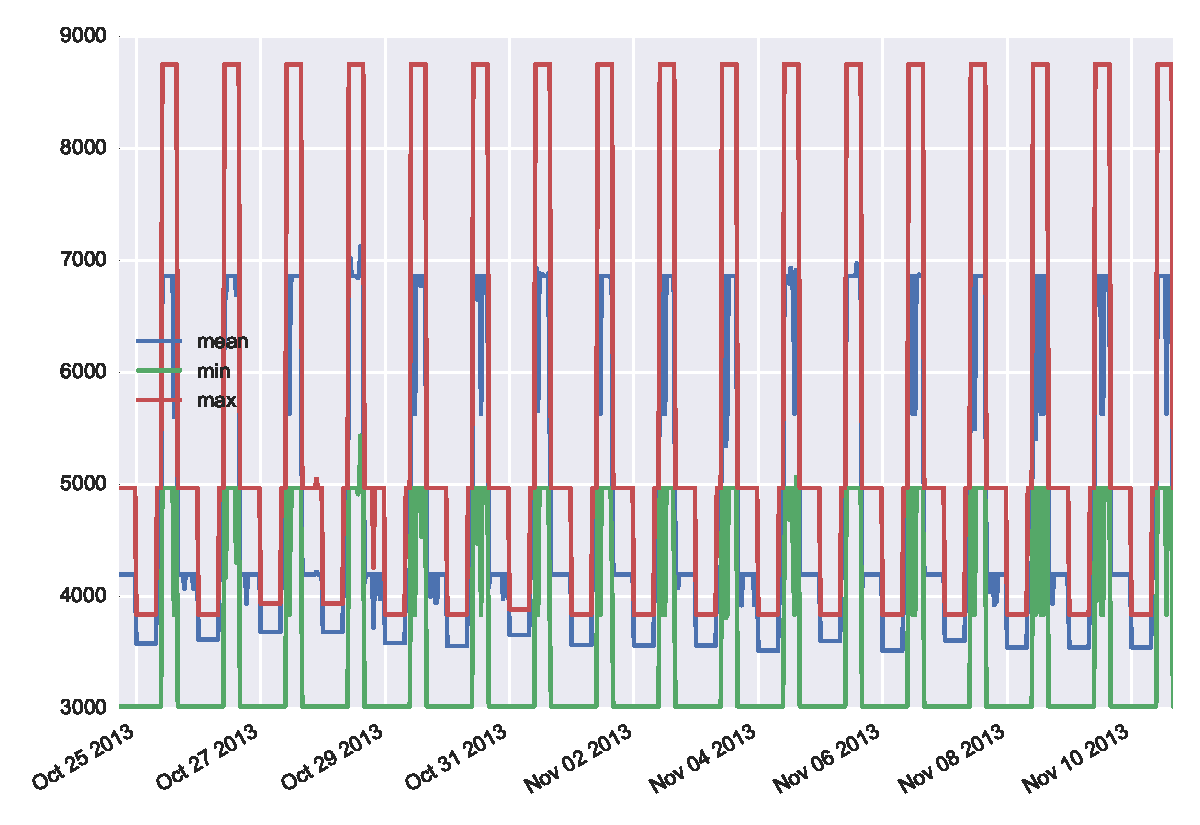
\includegraphics[width=\textwidth]{adjusted_sums_summary.pdf}
		\caption{A summary of the summation of all fumehood and laboratory evacuation over time across the different parameters evaluated.  Significant dips in evacuation are typically night time.}
	\end{figure*}
	

\section{Conclusion}

\end{document}